
\begin{frame}{What is EULA (End User License Agreement)?}
  \begin{itemize}
    \item A legal contract between the software developer and the end user.
    \item Grants the user the right to use the software under specific terms.
    \item Often displayed during installation or first launch.
    \item Typically non-negotiable ("take-it-or-leave-it")\cite{DEFINITION}.
  \end{itemize}
\end{frame}

\begin{frame}{EULA vs. Terms of Service (ToS)}
  \begin{table}[h!]
    \centering
    \begin{tabular}{|l|p{5cm}|p{7cm}|}
    \hline
    \textbf{Aspect} & \textbf{EULA} & \textbf{Terms of Service (ToS) / Terms \& Conditions (T\&C)} \\
    \hline
    \textbf{Scope} & Focused on \textbf{software usage rights} & Broader: website, service, and platform rules \\
    \hline
    \textbf{Target} & Individual \textbf{software users} & Website/app users, consumers, community members \\
    \hline
    \textbf{Binding} & Usually shown during installation & Often on websites (agreed via use) \\
    \hline
    \textbf{Example} & Microsoft Windows EULA & Facebook Terms of Service \\
    \hline
    \end{tabular}
    \caption{Comparison between EULA and Terms of Service\cite{TOS}}
  \end{table}
\end{frame}

\begin{frame}{Why are EULAs Rarely Read?}
    \begin{itemize}
      \item Too long and full of legal jargon.
      \item Presented during moments when users are eager to proceed (e.g., install).
      \item Click-through agreements make it easy to skip reading.
      \item Psychological: “Everyone else accepts, so I do too.”\cite{RARE}
    \end{itemize}
    \begin{alertblock}{Interesting fact}
      A study by Carnegie Mellon University estimated that reading all the privacy policies encountered annually would take the average user 76 workdays\cite{FACT}.
    \end{alertblock}
\end{frame}

\begin{frame}{Why are EULAs Rarely Read?}
\begin{columns}[c]
    \column{.5\textwidth}
    \centering
    \begin{figure}
        \centering
        
\includegraphics[width=0.65\textwidth]{images/dog.png}
        \label{fig:dog}
    \end{figure}  
    \column{.5\textwidth}
    \centering
    \begin{figure}
        \centering
        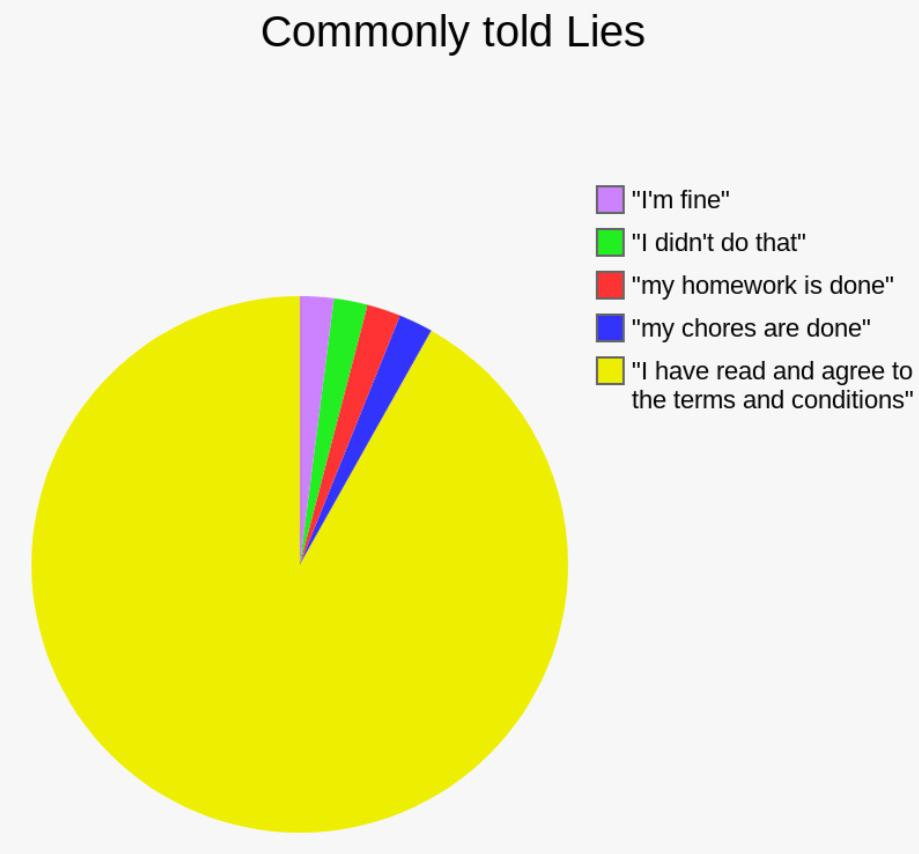
\includegraphics[width=\textwidth]{images/lies.jpg}
        \label{fig:lies}
    \end{figure}    
\end{columns}
\end{frame}
